\documentclass[11pt,a4paper]{report}%especifica o tipo de documento que tenciona escrever: carta, artigo, relatório... neste caso é um relatório
% [11pt,a4paper] Define o tamanho principal das letras do documento. caso não especifique uma delas, é assumido 10pt
% a4paper -- Define o tamanho do papel.
\usepackage{float}
\usepackage[portuges]{babel}%Babel -- irá activar automaticamente as regras apropriadas de hifenização para a língua todo o
                                   %-- o texto gerado é automaticamente traduzido para Português.
                                   %  Por exemplo, “chapter” irá passar a “capítulo”, “table of contents” a “conteúdo”.
                                   % portuges -- específica para o Português.
\usepackage[utf8]{inputenc} % define o encoding usado texto fonte (input)--usual "utf8" ou "latin1

\usepackage{graphicx} %permite incluir graficos, tabelas, figuras
\usepackage{url} % para utilizar o comando \url{}
\usepackage{enumerate} %permite escolher, nas listas enumeradas, se os iems sao marcados com letras ou numeros-romanos em vez de numeracao normal

%\usepackage{apalike} % gerar biliografia no estilo 'named' (apalike)

\usepackage{color} % Para escrever em cores

\usepackage{multirow} %tabelas com multilinhas
\usepackage{array} %formatação especial de tabelas em array

\usepackage[pdftex]{hyperref} % transformar as referências internas do seu documento em hiper-ligações.

%Exemplos de fontes -- nao e vulgar mudar o tipo de fonte
%\usepackage{tgbonum} % Fonte de letra: TEX Gyre Bonum
%\usepackage{lmodern} % Fonte de letra: Latin Modern Sans Serif
%\usepackage{helvet}  % Fonte de letra: Helvetica
%\usepackage{charter} % Fonte de letra:Charter

\definecolor{saddlebrown}{rgb}{0.55, 0.27, 0.07} % para definir uma nova cor, neste caso 'saddlebrown'

\usepackage{listings}  % para utilizar blocos de texto verbatim no estilo 'listings'
%paramerização mais vulgar dos blocos LISTING - GENERAL
\lstset{
	basicstyle=\small, %o tamanho das fontes que são usadas para o código
	numbers=left, % onde colocar a numeração da linha
	numberstyle=\tiny, %o tamanho das fontes que são usadas para a numeração da linha
	numbersep=5pt, %distancia entre a numeração da linha e o codigo
	breaklines=true, %define quebra automática de linha
    frame=tB,  % caixa a volta do codigo
	mathescape=true, %habilita o modo matemático
	escapeinside={(*@}{@*)} % se escrever isto  aceita tudo o que esta dentro das marcas e nao altera
}
%
%\lstset{ %
%	language=Java,							% choose the language of the code
%	basicstyle=\ttfamily\footnotesize,		% the size of the fonts that are used for the code
%	keywordstyle=\bfseries,					% set the keyword style
%	%numbers=left,							% where to put the line-numbers
%	numberstyle=\scriptsize,				% the size of the fonts that are used for the line-numbers
%	stepnumber=2,							% the step between two line-numbers. If it's 1 each line
%											% will be numbered
%	numbersep=5pt,							% how far the line-numbers are from the code
%	backgroundcolor=\color{white},			% choose the background color. You must add \usepackage{color}
%	showspaces=false,						% show spaces adding particular underscores
%	showstringspaces=false,					% underline spaces within strings
%	showtabs=false,							% show tabs within strings adding particular underscores
%	frame=none,								% adds a frame around the code
%	%abovecaptionskip=-.8em,
%	%belowcaptionskip=.7em,
%	tabsize=2,								% sets default tabsize to 2 spaces
%	captionpos=b,							% sets the caption-position to bottom
%	breaklines=true,						% sets automatic line breaking
%	breakatwhitespace=false,				% sets if automatic breaks should only happen at whitespace
%	title=\lstname,							% show the filename of files included with \lstinputlisting;
%											% also try caption instead of title
%	escapeinside={\%*}{*)},					% if you want to add a comment within your code
%	morekeywords={*,...}					% if you want to add more keywords to the set
%}

\usepackage{xspace} % deteta se a seguir a palavra tem uma palavra ou um sinal de pontuaçao se tiver uma palavra da espaço, se for um sinal de pontuaçao nao da espaço

\parindent=0pt %espaço a deixar para fazer a  indentação da primeira linha após um parágrafo
\parskip=2pt % espaço entre o parágrafo e o texto anterior

\setlength{\oddsidemargin}{-1cm} %espaço entre o texto e a margem
\setlength{\textwidth}{18cm} %Comprimento do texto na pagina
\setlength{\headsep}{-1cm} %espaço entre o texto e o cabeçalho
\setlength{\textheight}{23cm} %altura do texto na pagina

% comando '\def' usado para definir abreviatura (macros)
% o primeiro argumento é o nome do novo comando e o segundo entre chavetas é o texto original, ou sequência de controle, para que expande
\def\darius{\textsf{Darius}\xspace}
\def\antlr{\texttt{AnTLR}\xspace}
\def\pe{\emph{Publicação Eletrónica}\xspace}
\def\titulo#1{\section{#1}}    %no corpo do documento usa-se na forma '\titulo{MEU TITULO}'
\def\super#1{{\em Supervisor: #1}\\ }
\def\area#1{{\em \'{A}rea: #1}\\[0.2cm]}
\def\resumo{\underline{Resumo}:\\ }

%\input{LPgeneralDefintions} %permite ler de um ficheiro de texto externo mais definições

\title{Trabalho Teórico 1 de Arquiteturas Aplicacionais\\
        1º/4º ano MEI/MIEI\\
       \textbf{Frameworks Java e .NET}\\ Relatório de Desenvolvimento
       } %Titulo do documento
%\title{Um Exemplo de Artigo em \LaTeX}
\author{João Paulo Oliveira de Andrade Marques \\ (a81826@alunos.uminho.pt) \and José André Martins Pereira\\ (a82880@alunos.uminho.pt) \and Ricardo André Gomes Petronilho\\ (a81744@alunos.uminho.pt)
       } %autores do documento
\date{\today} %data

\usepackage[dvipsnames]{xcolor}



\usepackage{hyperref}
\hypersetup{
    colorlinks=true,
    linkcolor=blue,
    filecolor=magenta,      
    urlcolor=cyan,
}



\begin{document} % corpo do documento

\begin{figure}
    \centering
    
\includegraphics{images/uminho.png}
\end{figure}

\maketitle % apresentar titulo, autor e data

\tableofcontents % Insere a tabela de indice
\listoffigures % Insere a tabela de imagens

\section{Introdução}
\label{sec:introducao}

\hspace{5mm} O presente relatório relata a investigação sobre \textbf{Design Patterns} no âmbito da Unidade Curricular Arquitecturas Aplicacionais do 4º ano do Mestrado integrado em Engenharia Informática da Universidade do Minho.

\hspace{2mm} O grupo de trabalho decidiu apresentar dois Design Patterns, sendo estes: o \textbf{Memento} e o \textbf{Observer}.

% \hspace{2mm} Primeiro será ilustrado o \textbf{Memento} e de seguida o \textbf{Observer}.
\chapter{Frameworks}
\label{sec:frameworks}

Nesta secção serão apresentadas algumas das frameworks escolhidas pelo grupo para o trabalho a realizar.

% \section{Blade}
\label{sec:blade}

\begin{figure}[H]
    \centering
    
\includegraphics[scale=0.4]{images/blade.png}
    \caption{Logotipo da framework Blade.}
    \label{fig:blade}
\end{figure}

\hspace{5mm} A \textbf{Blade} consiste numa framework web (JavaWeb) simples/eficiente, onde as suas principais características no desenvolvimento são a performance e flexibilidade. 

\hspace{5mm} Do mesmo modo, esta framework também se caracteriza pela sua simplicidade, pois segundo os desenvolvedores da mesma, os utilizadores compreendem a \textbf{Blade} num único dia. A simplicidade deve-se ao facto de a framework não introduzir vários níveis entre o utilizador e as bibliotecas \textit{standard}.

\hspace{5mm} A framework \textbf{Blade} segue a arquitetura MVC (Model-View-Controller)

\hspace{5mm} As figuras seguintes (\ref{fig:blade-1},\ref{fig:blade-2},\ref{fig:blade-3} e \ref{fig:blade-4}), representam um \textit{Quick Start}, que pode ser consultado na página do GitHub da framework \textcolor{blue}{\textbf{\href{https://github.com/lets-blade/blade}{Blade}}}. Neste \textit{Quick Start}, abordam-se as capacidades da framework para a criação de aplicações web, monitorização do servidor e output (\textit{view}) dessa mesma aplicação.

\begin{figure}[H]
    \centering
    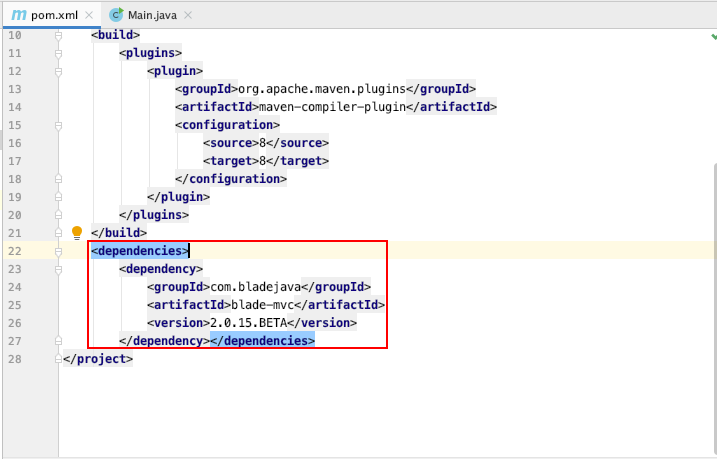
\includegraphics[scale=0.5]{images/blade-1.png}
    \caption{Ficheiro Maven com as dependências necessárias para utilização da framework \textbf{Blade} para este \textit{Quick Start}.}
    \label{fig:blade-1}
\end{figure}

\begin{figure}[H]
    \centering
    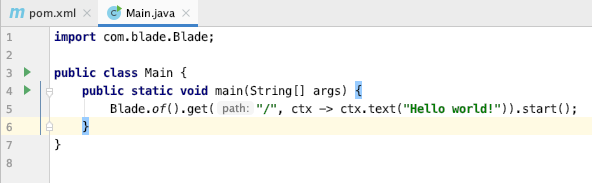
\includegraphics[scale=0.6]{images/blade-2.png}
    \caption{Código Java para \textit{Quick Start}.}
    \label{fig:blade-2}
\end{figure}

\begin{figure}[H]
    \centering
    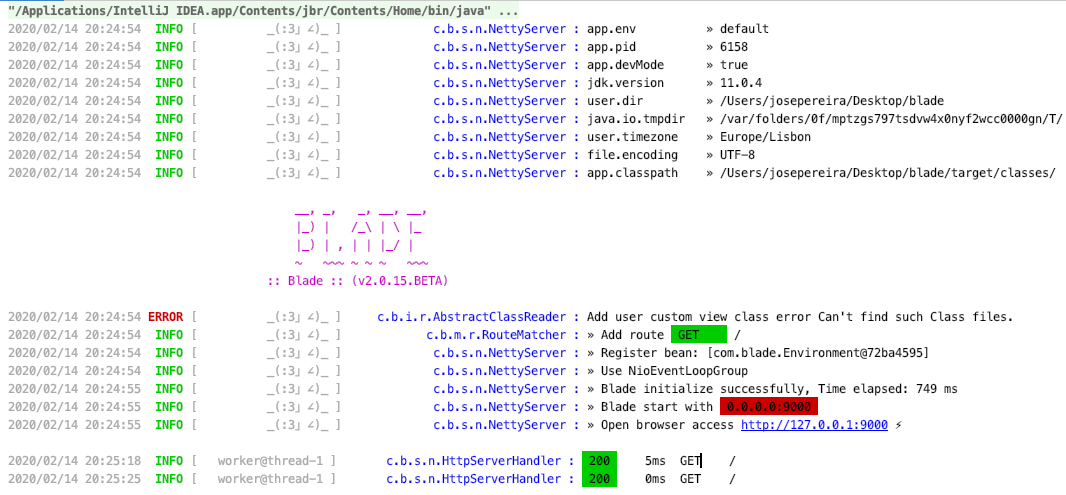
\includegraphics[scale=0.4]{images/blade-3.png}
    \caption{Monitorização do servidor web, fornecida pela framework \textbf{Blade}, onde se pode ver os pedidos.}
    \label{fig:blade-3}
\end{figure}

\begin{figure}[H]
    \centering
    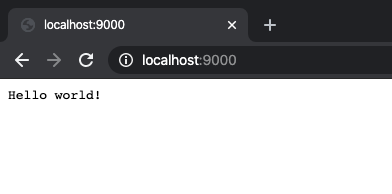
\includegraphics[scale=0.6]{images/blade-4.png}
    \caption{A aplicação web criada pela framework.}
    \label{fig:blade-4}
\end{figure}
\section{Grails}
\label{subsec:grails}

\begin{figure}[H]
    \centering
    
\includegraphics[scale=0.27]{images/grails.png}
    \caption{Logotipo da framework Grails.}
    \label{fig:grails}
\end{figure}

\hspace{5mm} As frameworks web mais recentes tendem a ser bastante complicadas/complexas do que o necessário. 

\hspace{5mm} Desta forma, a \textbf{Grails}, acenta no conceito de framework dinâmica, tal como \textbf{Rails} e \textbf{Django}, tendo como principal objetivo, a simplicidade, reduzindo a complexidade da construção de aplicações web na plataforma Java.

\hspace{5mm} A escolha desta framework para este trabalho, deveu-se ao facto da mesma centrar-se também na separação de camadas de uma aplicação web, reduzindo as preocupações do densenvolvedor.

\hspace{5mm} A framework segue uma arquitetura full stack, isto é, híbrida (\textit{server side} e \textit{client side}), abrangindo todas as camadas de uma aplicação web. No entanto, o grupo focou-se mais nas camadas MVC (Model View and Controller), da camada de apresentação.

\hspace{5mm} A \textit{Groovy} é a linguagem de programação utilizada na framework, sendo esta orientada a objetos, desenvolvida para a plataforma \textit{Java}, como  alternativa à mesma. A linguagem  caracteriza-se por ser bastante semelhante, a nível de sintax, a \textit{Python}, \textit{Ruby}, entre outras. Desta forma, sendo desenvolvida para a plataforma Java, a framework \textbf{Grails}, como utiliza esta linguagem, considera-se uma framework da plataforma Java, tal como os próprios desenvolvedores o afirmam.

\hspace{5mm} A framework \textbf{Grails} contém um interpretador/aplicação interativo (que será mostrado de seguida em detalhe), onde se controla toda a estrutura da aplicação web, e desta forma, a framework consegue organizar o projeto, separando as várias camadas sem intrevenção do desenvolvedor, de forma automática.

\hspace{5mm} Com o objetivo de uma melhor perceção de como a framework \textbf{Grails} efetua a separação de camadas \textbf{MVC}, vai-se apresentar um exemplo prático simples, que o grupo fez para melhor entender a mesma.

\hspace{5mm} Após a instalação dos requisitos (Java 8+, Grails), executa-se o comando \textit{grails create-app nome-app} (figura \ref{fig:grails-1}), para a criação da estrutura do projeto, com todas os ficheiros de configuração necessários, bem como, as diretorias das várias camadas e dependências, tal como se pode observar na figura \ref{fig:grails-2}.

\begin{figure}[H]
    \centering
    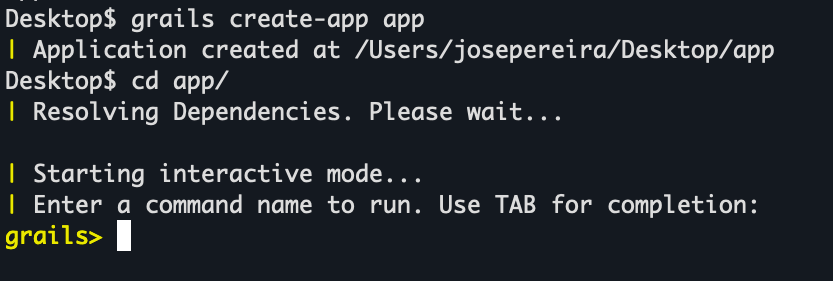
\includegraphics[scale=0.45]{images/grails-1.png}
    \caption{Criação da aplicação, e inicialização do interpretador da framework \textbf{Grails}.}
    \label{fig:grails-1}
\end{figure}

\begin{figure}[H]
    \centering
    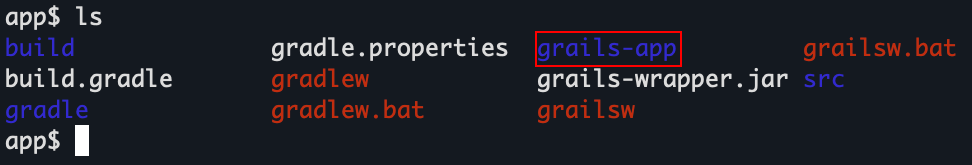
\includegraphics[scale=0.50]{images/grails-2.png}
    \caption{Estrutura do projeto criada após execução do comando \textit{grails create-app nome-app}.}
    \label{fig:grails-2}
\end{figure}

\hspace{5mm} Após a criação da aplicação, executa-se o comando \textit{grails}, para aceder ao interpretador. A execução da aplicação, faz-se através do interpretador, com o comando \textit{run-app}, tal como se pode observar na figura \ref{fig:grails-6}. A aplicação acede-se via browser no \textit{localhost}, porta 8080, onde aparecerá, uma página da \textit{Grails}, sendo possível ver os controllers existentes, tal como se pode observar na figura \ref{fig:grails-7}. 


\begin{figure}[H]
    \centering
    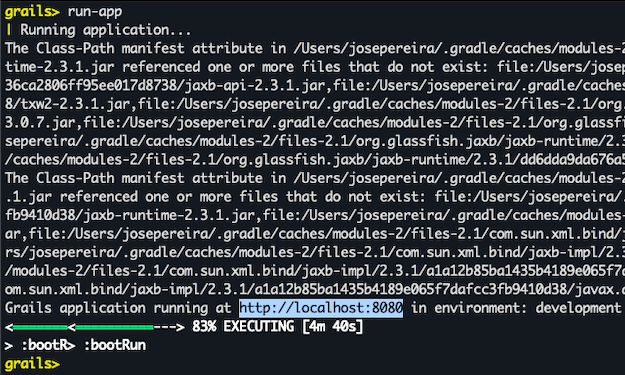
\includegraphics[scale=0.50]{images/grails-6.png}
    \caption{Execução da aplicação web, através do interpretador.}
    \label{fig:grails-6}
\end{figure}

\hspace{5mm} A diretoria mais importante é a \textit{graisl-app}, onde se encontram todos os sources files \textbf{Grovvy}. Nesta diretoria, os ficheiros são divididos em diferentes sub-diretorias (camadas), de forma automática pela framework. Na figura \ref{fig:grails-3}, pode-se verificar com mais detalhe a composição desta diretoria, onde se assinala a quadrados vermelhos as camadas \textbf{MVC}.

\begin{figure}[H]
    \centering
    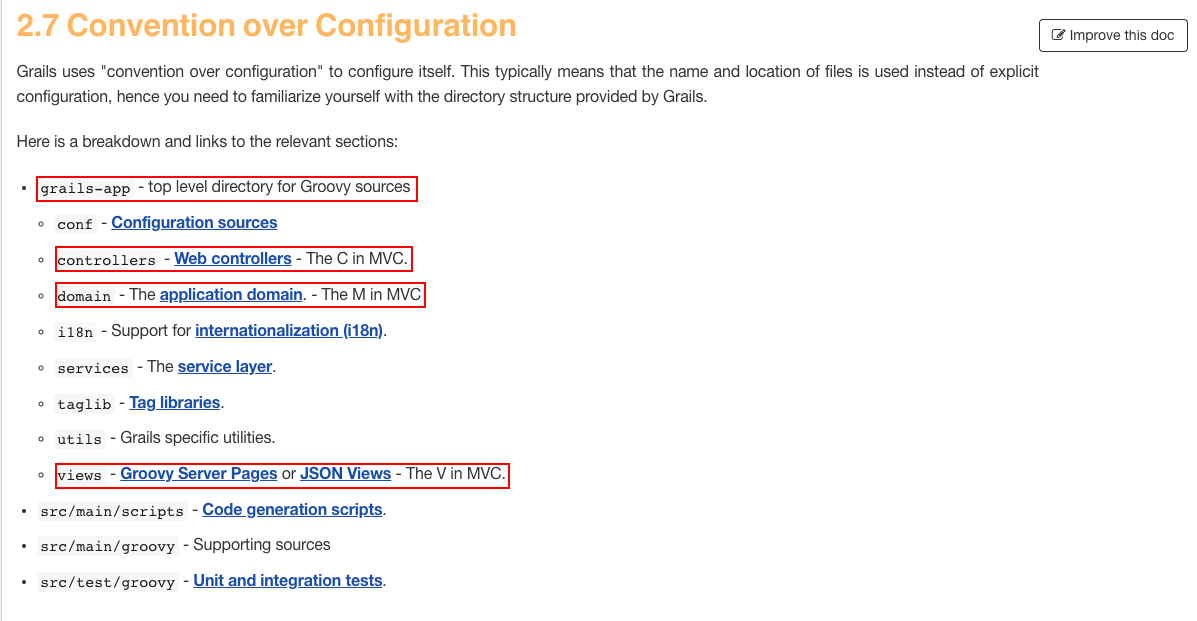
\includegraphics[scale=0.50]{images/grails-3.png}
    \caption{Composição da diretoria \textit{grails-app}, distribuindo as várias camadas, por diferentes diretorias.}
    \label{fig:grails-3}
\end{figure}

\hspace{5mm} No entanto, poderá-se pensar que o programador terá o trabalho de colocar os diferentes ficheiros, nas diferentes pastas. A resposta é "não", a própria framework tal como já foi dito, faz isso. Na verdade, para se criar um \textit{Controller}, faz-se através do interpretador (figura \ref{fig:grails-4}), e desta forma, a framework consegue controlar e organizar as diferentes camadas. 

\hspace{5mm} Após a criação do controlador, é criada a classe do mesmo, na diretoria \textit{controllers}, com o sufixo \textit{Controller} ao nome dado na criação. A classe gerada, contém um método padrão, denominado \textit{index}, que corresponde a uma ação (figura \ref{fig:grails-5}), sendo que um controlador pode ter várias ações, ou seja, vários métodos.  

\begin{figure}[H]
    \centering
    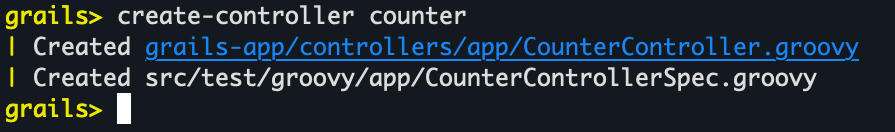
\includegraphics[scale=0.50]{images/grails-4.png}
    \caption{Criação do controller denominado \textit{Counter}.}
    \label{fig:grails-4}
\end{figure}

\begin{figure}[H]
    \centering
    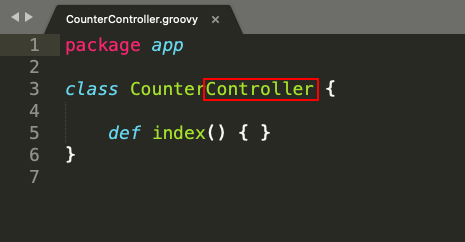
\includegraphics[scale=0.50]{images/grails-5.png}
    \caption{Classe criada automaticamente pela framework, onde é adicionado um sufixo de \textit{Controller} e um método padrão, denominado index.}
    \label{fig:grails-5}
\end{figure}

\hspace{5mm} A seguir, à criação do controlador, o mesmo já fica visível na homepage da aplicação web (figura \ref{fig:grails-7}). A forma de aceder ao controlador e às respetivas ações, segue o seguinte padrão http://localhost:8080/\textcolor{red}{controller-name}/\textcolor{blue}{action} (no caso de argumentos http://localhost:8080/\textcolor{red}{controller-name}/\textcolor{blue}{action}?agr1=value1).

\hspace{5mm} Daqui advém, os pontos fortes desta framework, para além da separação das camadas MVC, vistas anteriormente, a redução da complexidade, pois compara-se o nome do URL, com o nome do método, sabendo o método a executar, não sendo necessárias anotações ou outras alternativas, presentes em outras frameworks. Do mesmo modo, pedidos do tipo \textbf{GET} com argumentos, também se tornam simples, pois basta o método receber os argumentos com o mesmo nome dado no URL, tal como se pode observar na figura \ref{fig:grails-8} e \ref{fig:g-4} da ação \textit{set}.

\begin{figure}[H]
    \centering
    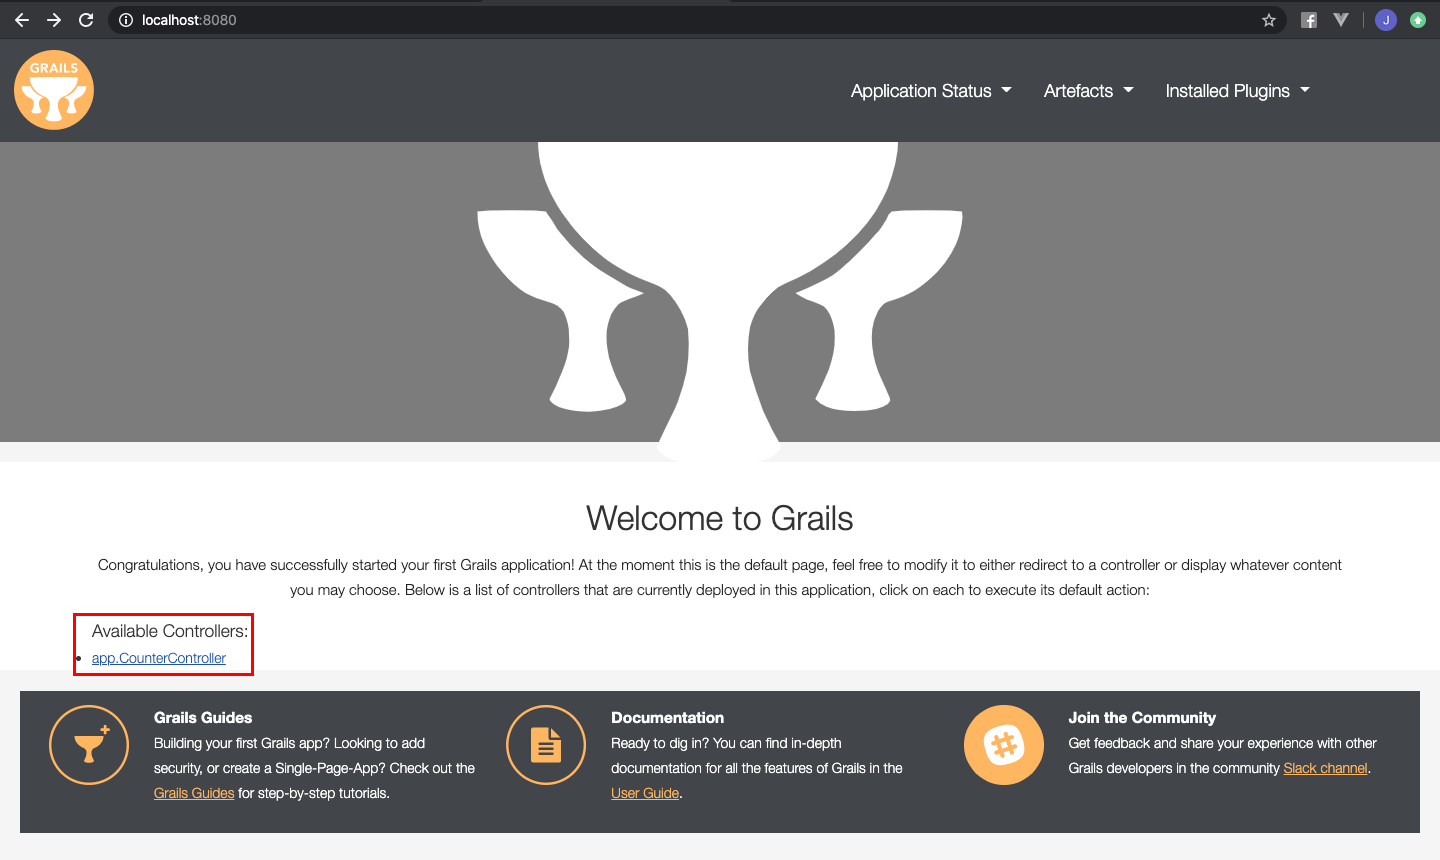
\includegraphics[scale=0.30]{images/grails-7.png}
    \caption{Aplicação web, página inicial, com lista de controllers disponíveis.}
    \label{fig:grails-7}
\end{figure}

\hspace{5mm} Assim, após a perceção do funcionamento dos controllers, desenvolvemos várias ações para o mesmo controller, tal como se pode verificar, na figura \ref{fig:grails-8}.

\hspace{5mm} Importante realçar que o método \textit{render}, envia as strings ou valores para uma view criada automaticamente, caso esta ainda não exista, ou seja, a framework abstrai o desenvolvedor desse processo, tornando-o simples. De seguida, apresentamos os vários outputs para as diversas ações definidas, nas figuras, \ref{fig:g-1}, \ref{fig:g-2}, \ref{fig:g-3} e \ref{fig:g-4}.

\begin{figure}[H]
    \centering
    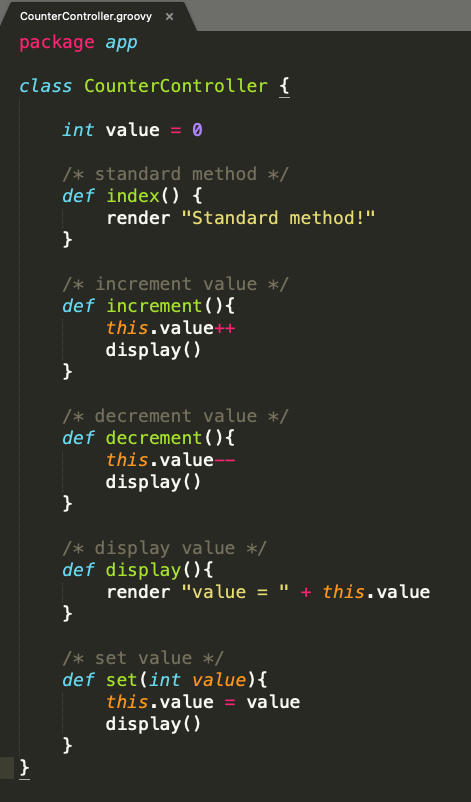
\includegraphics[scale=0.50]{images/grails-8.png}
    \caption{Controller com mais ações definidas.}
    \label{fig:grails-8}
\end{figure}

\begin{figure}[H]
    \centering
    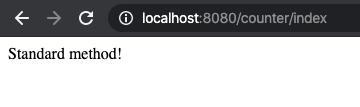
\includegraphics[scale=0.50]{images/g-1.png}
    \caption{Execução da ação index.}
    \label{fig:g-1}
\end{figure}

\begin{figure}[H]
    \centering
    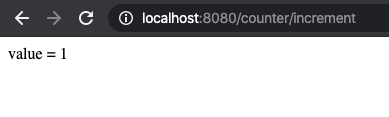
\includegraphics[scale=0.50]{images/g-2.png}
    \caption{Execução da ação increment.}
    \label{fig:g-2}
\end{figure}

\begin{figure}[H]
    \centering
    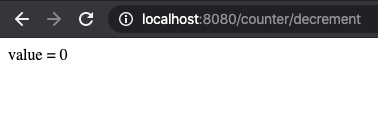
\includegraphics[scale=0.50]{images/g-3.png}
    \caption{Execução da ação decrement.}
    \label{fig:g-3}
\end{figure}

\begin{figure}[H]
    \centering
    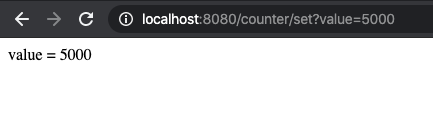
\includegraphics[scale=0.50]{images/g-4.png}
    \caption{Execução da ação set.}
    \label{fig:g-4}
\end{figure}

\hspace{5mm} Assim, conclui-se em relação à framework \textbf{Grails}, que faz uma boa divião das camadas MVC, bem como de outros níveis da aplicação, tornando-as independentes. Também importante realçar a característica de redução de complexidade e simplicidade desta framework.






\section{GWT}
\label{subsec:gwt}

\begin{figure}[H]
    \centering
    
\includegraphics[scale=0.15]{images/gwt.png}
    \caption{Logotipo da framework GWT.}
    \label{fig:gwt}
\end{figure}

\hspace{5mm} A \href{http://www.gwtproject.org/}{\textbf{GWT}} consiste numa framework para construir e otimizar aplicações web complexas.

\hspace{5mm} Esta framework foi criada pela Google com o intuito de ser simples para os programadores desenvolverem a aplicação web e ser muito eficiente para os utilizadores. É uma framework client-side, apesar de ter um servidor a correr, este apenas serve para disponibilizar a view. Além disso esta framework não segue o modelo \textbf{MVC}, mas sim o modelo \textbf{MVP} (Model-View-Presenter).

\hspace{5mm} O \textbf{MVP} consiste em o utilizador interagir com a View, esta notifica o Presenter que por sua vez atualiza o Model, de seguida o Presenter obtém dados do Model e encaminha-os para a View para esta ser atualizada. A seguinte figura ilustra o funcionamento do modelo \textbf{MVP}.

\begin{figure}[H]
    \centering
    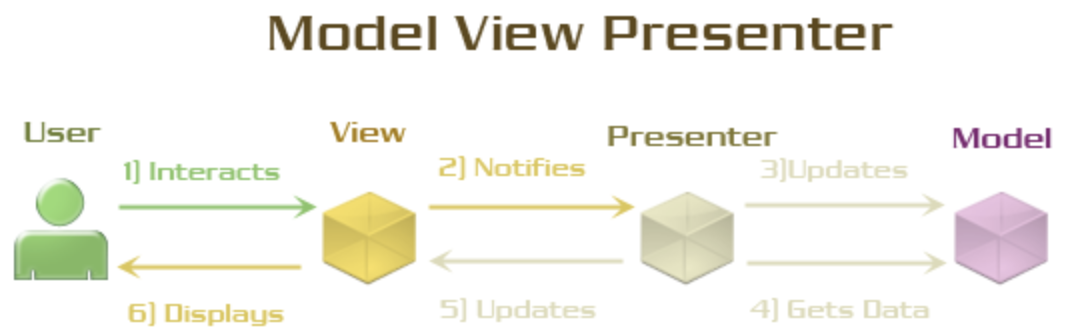
\includegraphics[scale=0.75]{images/MVP.png}
    \caption{Modelo \textbf{MVP}.}
    \label{fig:MVP}
\end{figure}

\hspace{5mm} Algumas das vantagens de utilizar o \textbf{GWT}:
\begin{itemize}
    \item Fornece API's Java e Widgets que permitem a escrita de aplicações AJAX em Java que depois são compiladas para JavaScript;
    \item Permite a colocação de "split-points" no código o que fará com que aplicações muito grandes possam ser divididas em vários segmentos JavaScript para um arranque mais rápido da página Web enquanto descarrega o resto dos fragmentos;
    \item Possui duas ferramentas de otimização para que o JavaScript gerado através do Java seja o mais eficiente possível, mas que também evite incompatibilidades entre diversos browsers;
    \item Os erros são encontrados em tempo de compilação;
    \item Pode ainda ser utilizado JavaScript entre o código Java através do JSNI (JavaScript Native Interface).
\end{itemize}

\hspace{5mm} De seguida será ilustrado um pequeno exemplo para mostrar a simplicidade da framework.

\begin{figure}[H]
    \centering
    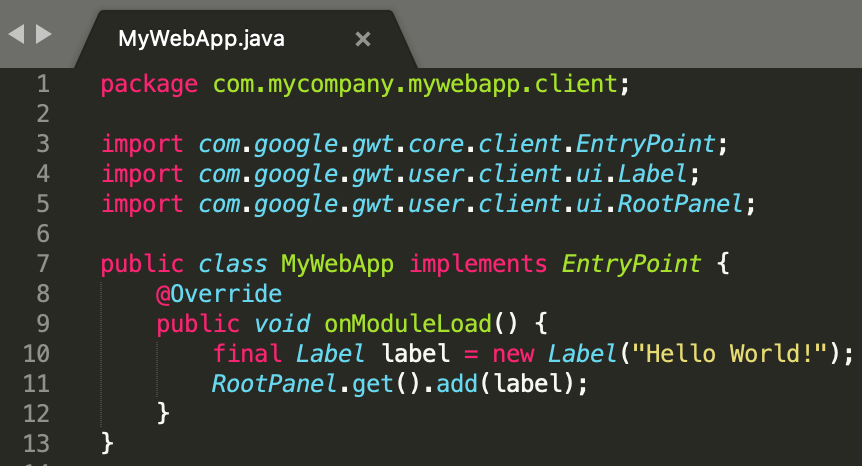
\includegraphics[scale=0.7]{images/gwt-1.png}
    \caption{Código Java para \emph{Quick Start}.}
    \label{fig:gwt-1}
\end{figure}

\begin{figure}[H]
    \centering
    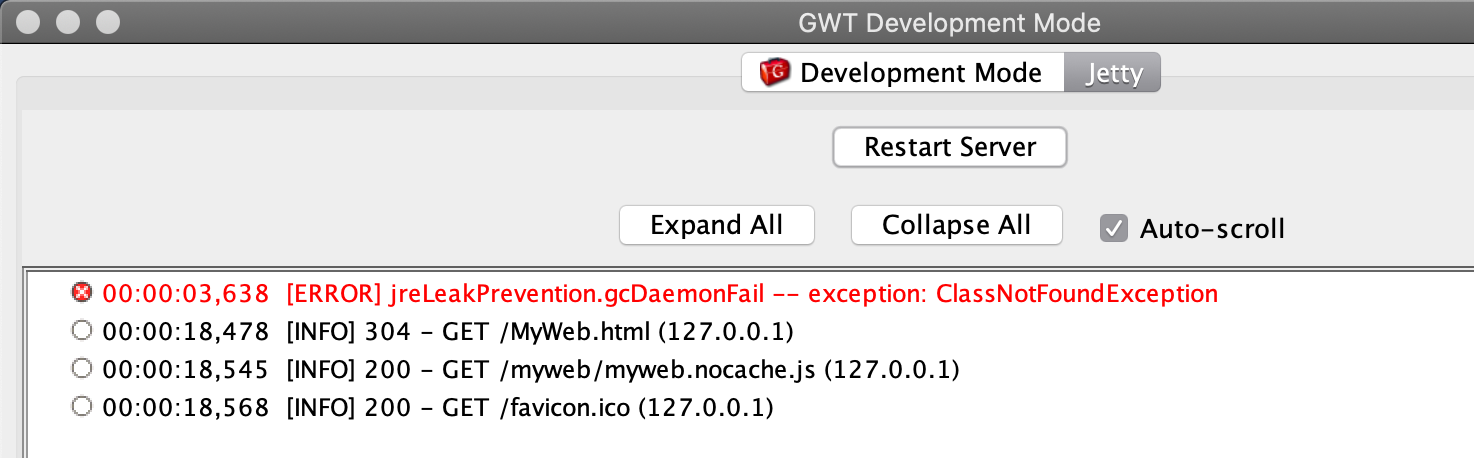
\includegraphics[scale=0.5]{images/gwt-2.png}
    \caption{Monitorização do servidor web, fornecida pela framework \textbf{GWT}, onde se pode ver os pedidos.}
    \label{fig:gwt-2}
\end{figure}

\begin{figure}[H]
    \centering
    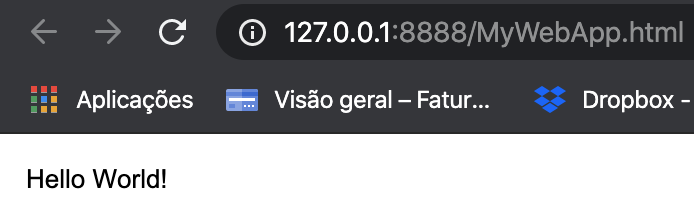
\includegraphics[scale=0.8]{images/gwt-3.png}
    \caption{A aplicação web criada pela framework.}
    \label{fig:gwt-3}
\end{figure}
% \section{Hibernate}
\label{subsec:hibernate}

\begin{figure}[H]
    \centering
    
\includegraphics[scale=0.25]{images/hibernate.jpg}
    \caption{Logotipo da framework Hibernate.}
    \label{fig:hibernate}
\end{figure}

\href{http://hibernate.org/}{http://hibernate.org/}

\hspace{5mm} O \textbf{Hibernate} ...


Server side only
\section{Spring}
\label{subsec:spring}

\begin{figure}[H]
    \centering
    
\includegraphics[scale=0.11]{images/spring.png}
    \caption{Logotipo da framework Spring.}
    \label{fig:spring}
\end{figure}

\hspace{5mm} A \href{https://spring.io/}{Spring} é uma framework desenvolvida pela equipa \href{https://pivotal.io/}{pivotal} usando Java dedicada principalmente à implementação de lógica aplicacional back-end.

\subsection{Vanatagens}

\hspace{5mm} Existem enúmeras vantagens ao utilizar esta framework tais como:

\begin{itemize}
    
    \item é \textbf{escrita em Java}, beneficiando do facto de ser uma linguaguem muito usada e preparada para projetos de elevada complexidade (usando conceitos de POO). Outra vantagem da utilização de Java é a comunidade (tanto documentação oficial como tutoriais e explicações de terceiros) ser grande e consistente, tornando o suporte a dúvidas e obstáculos do desenvolvimento mais facilitados de se superar.
    
    \item diversos desenvolvedores fidedignos, tais como: Alibaba, Amazon, Google, Microsoft, entre outros; \textbf{confiam na framework}, sendo um indicador positivo a favor da utilização da mesma. 
    
    \item é uma framework \textbf{flexivel} uma vez que a sua arquitetura base utiliza os padrões \href{https://en.wikipedia.org/wiki/Inversion_of_control}{Inversion of Control (IoC)} e \href{https://en.wikipedia.org/wiki/Dependency_injection}{Dependency Injection (DI)} tornando a implementação do código facilitada uma vez que parte considerável da lógica é automaticamente introduzida.
    
    \item contém inúmeras \textbf{bibliotecas de terceiros} integradas na arquitetura base constituindo um conjunto de ferramentas disponível para qualquer tipo de aplicação tanto server-side como client-side. Por exemplo a framework \href{https://hibernate.org/}{hibernate} é facilmente integrada no modelo de dados de uma API RESTful já escrita em Spring, tornando o processo de presistência de dados intuitivo e praticamente automático.  
    
    \item contém o \textbf{plugin} \href{https://spring.io/projects/spring-boot}{Spring boot} que automatiza a criação da infaestrutura inicial do projeto: inicializando e configurando o servidor aplicacional \href{http://tomcat.apache.org/Tomcat}{Tomcat}, verifica e descarrega bibliotecas necessárias para o contexto da aplicação e disponibiliza métricas para avaliar o desempenho e estado do sistema, podendo ser remotamente avaliado.
    
    \item é uma framework \textbf{segura}. Utilizar bibliotecas de terceiros é sempre um risco uma vez que os seus desenvolvedores podem simplesmente desistir e descontinuar atualizações das bibliotecas ficando as mesmas sem suporte e sujeitas a vulnerabilidades ou erros. Desta forma a equipa da Spring monotoriza e verifica o estado das bibliotecas terceiras integradas na sua arquitetura certificando que o seu uso é seguro.
    
    \item por último mas não menos importante a Spring, tal como Java, tem uma \textbf{comunidade grande e prestável} com ínumeros tutoriais e artigos na própria documentação oficial.
\end{itemize}


\subsection{Arquitetura}

\begin{figure}[H]
    \centering
    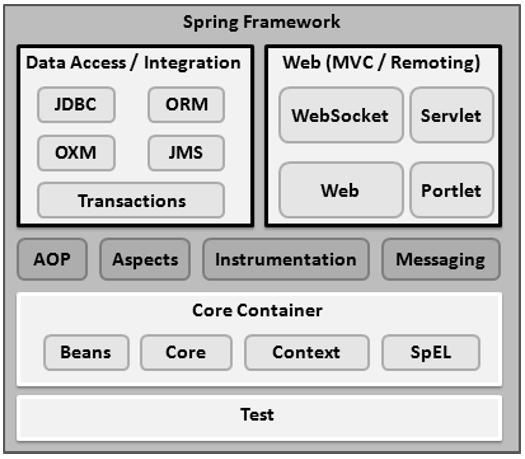
\includegraphics[scale=0.8]{images/spring_architecture.png}
    \caption{Arquitetura da framework Spring.}
    \label{fig:grails}
\end{figure}

\subsubsection{Core Container}

\hspace{5mm} O Core Container contém as principais classes que formam a arquitetura base da framework.

\begin{itemize}
    
    \item O módulo Core contém a implementação dos padrões arquiteturais: IoC e DI; referidos anteriormente.
    
    \item O módulo Bean implementa o padrão Factory (usado para criação genérica de obejtos), neste caso é uma fábrica de Beans.
    
    \item O módulo Context utiliza os módulos Core e Bean para gerar automaticamente os objetos configurados pela implementação específica do programador. 
    
    \item O módulo SpEL é utilizado pela Spring para gerar gráficos e monotorizar os objetos gerados e configurados pela própria framework.
    
\end{itemize}

\subsubsection{Outros Containers}

\hspace{5mm} O container Data Access implementa as classes necessárias ao acesso e manipulação de dados nas diferentes base de dados existentes.

\hspace{5mm} O container Web implementa o padrão MVC utilizado para responder a pedidos HTTP ou outros protocolos.


\subsection{Exemplo prático}

\hspace{5mm} Nesta secção segue-se um exemplo prático no qual foi criada uma API RESTful expondo a lógica back end através de métodos HTTP.

\subsubsection{Model - classe Person}

\hspace{5mm} Incialmente definiu-se uma classe Person que representa a informação de uma Pessoa, contendo o seu id, nome, idade e email. A vermelho em cima da declaração de cada variével de instância é possível observar \textbf{anotações}. 

\begin{figure}[H]
    \centering
    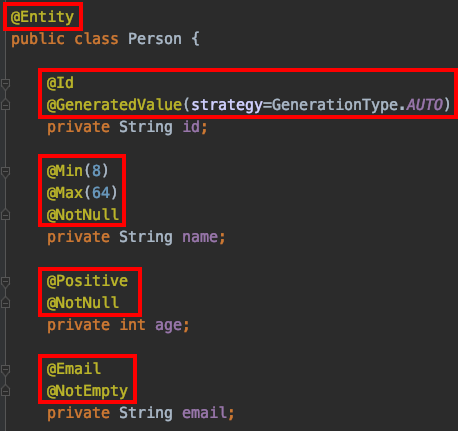
\includegraphics[scale=0.6]{images/Person_variables.png}
    \caption{Model Person.}
    \label{fig:grails}
\end{figure}

\begin{itemize}
    
    \item @GeneratedValue(...) - indica que a variável id é gerada automaticamente pela framework, neste caso é uma sequência de inteiros começado em 1 em formato String.
    
    \item @Min(8) - indica que a string (nome) tem de ter no mínimo 8 caracteres.
    
    \item @Max(64) - indica que a string (nome) tem de ter no máximo 64 caracteres.
    
    \item @NotNull - indica que a variável tem de ter necessáriamente um valor.
    
    \item @NotEmpty - indica que a variável tem de ter necessáriamente um valor não vazio.
    
    \item @Positive - indica que o inteiro (idade) tem de ser positivo.
    
    \item @Email - indica que a string tem de ter um formato válido de email.
    
\end{itemize}

\hspace{5mm} Existem outras anotações o importante é que a Spring juntamente com a framework hibernate integrada, valida automaticamente os valores atribuídos no momento de criação do objeto Person, lançando uma excepção quando os mesmos são inválidos.

\hspace{5mm} A anotação \textbf{@Entity} indica á hibernate que a classe refere-se a uma tablela na base de dados. A anotação \textbf{@Id} indica que a variável id é chave primária nessa mesma tabela.

\subsubsection{Controller - classe PersonController}

\hspace{5mm} Tendo definido o modelo de dados (classe Person) é necessário definir a classe que implementa os métodos que processam, neste caso, os pedidos HTTP associados a este objeto, a classe PersonController.


\begin{figure}[H]
    \centering
    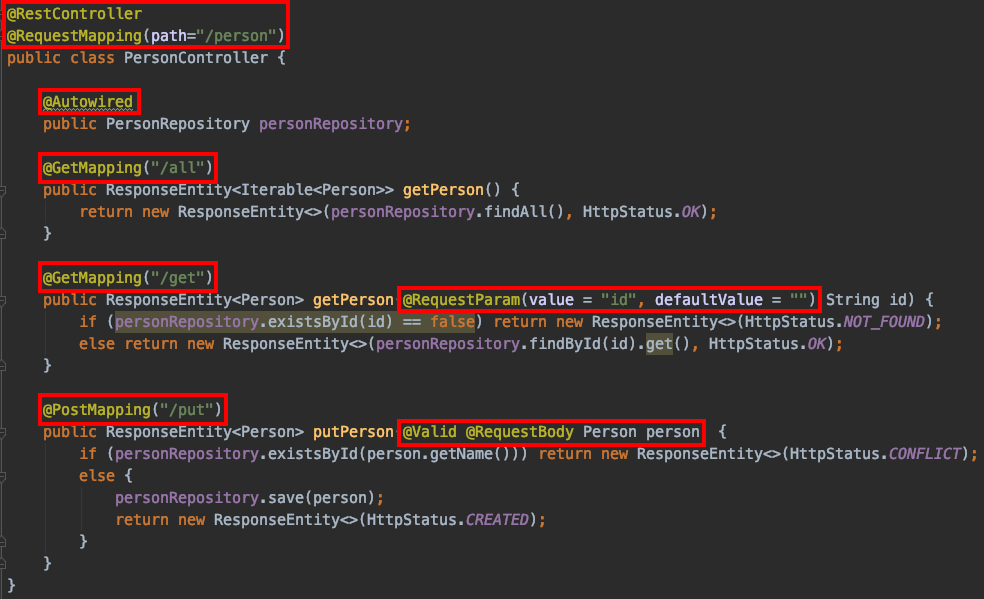
\includegraphics[scale=0.5]{images/PersonController.png}
    \caption{Controller PersonController.}
    \label{fig:grails}
\end{figure}

\begin{itemize}
    
    \item @RestController indica à Spring que esta classe é um Controller e por isso de acordo com o mapeamento das rotas pode processar HTTP Requests.
    
    \item RequestMapping(...) indica o nome da rota (no url) para evocar este controlador.
    
    \item @GetMapping(...) indica que este método processa HTTP GETs evocados pela rota definida no url.
    
    \item @PostMapping(...) indica que este método processa HTTP POSTs evocados pela rota definida no url.
    
    \item @Valid tal como referido anteriomente é utilizado para validar os dados introduzidos na classe model (neste caso Person). 
    
    \item @RequestBody indica que o objeto em causa foi exportado do payload (body) do pedido HTTP.
    
    \item @RequestParam indica que a variável em causa corresponde a um parâmetro específico do pedido HTTP.
    
    \item @Autowired é uma das anotações mais importante e eficaz, indica à framework hibernate que o objeto (neste caso PersonRepository) que é responsável pela persisntência dos dados (DAO) é automaticamente gerado e criado (criação dinâmica do objeto), sem qualquer intervenção do programador.
    
\end{itemize}

\subsubsection{DAO - interface PersonRepository}

\hspace{5mm} Esta interface provavelmente é a que demonstra de forma mais óbvia o poder de utilizar uma framework no sentido da \textbf{simplicidade e automação} de desenvolvimento de código.

\begin{figure}[H]
    \centering
    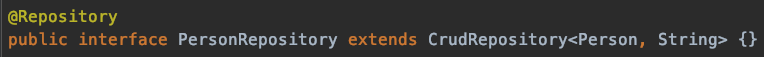
\includegraphics[scale=0.5]{images/PersonRepository.png}
    \caption{DAO PersonRepository.}
    \label{fig:grails}
\end{figure}

\hspace{5mm} Tal como se observa na figura, apenas indicando que a interface é do tipo CrudRepository e refere-se ao modelo de dados Person, a Spring juntamente com o Hibernate gera e cria dinâmicamente uma classe que implementa esta interface fazendo a ligação entre os modelos e a sua preseistência na base de dados.

\subsection{Análise final}

\hspace{5mm} Em suma, a criação das respetivas classes: Model, Controller e DAO; tornam-se simples e intuitiva uma vez que a Spring juntamente com as bibliotecas de terceiros integradas automatizam e gerem dinamicamente classes e dependências necessárias. 
% \section{Struts}
\label{subsec:struts}

\begin{figure}[H]
    \centering
    
\includegraphics[scale=0.25]{images/struts.png}
    \caption{Logotipo da framework Struts.}
    \label{fig:struts}
\end{figure}

\href{https://struts.apache.org/}{https://struts.apache.org/}

Existe uma segunda versão do Struts que é o Struts 2 podemos falar dela também.

Estou a ver também sobre esta, pq está relacionada com o spring. mas podem pesquisar tb e fazer merge de infos! ass José

\hspace{5mm} O \textbf{Struts} ...
\section{Conclusão}
\label{sec:conclusao}
\hspace{3mm} Após a conclusão desta pesquisa, percebe-se a utilidade do \textit{Dependency Injection} e \textit{Inversion of Control}, nas aplicações atuais, visto que estão em constante evolução. 

Tal como se viu ao longo deste relatório, estes \textit{patterns} caracterizam-se por facilitarem o processo de evolução de código, onde após alterações no mesmo, reduz-se a necessidade de serem alteradas outras partes.

Em relação ao \textit{Inversion of Control}, percebe-se a sua utilidade, visto que, se existir uma arquitectura previamente bem definida e comum a vários projectos, torna-se fácil a análise e trabalho sobre estes. 

\end{document}

